\section{Results}
\label{sec:results}

\begin{figure}
\centering
  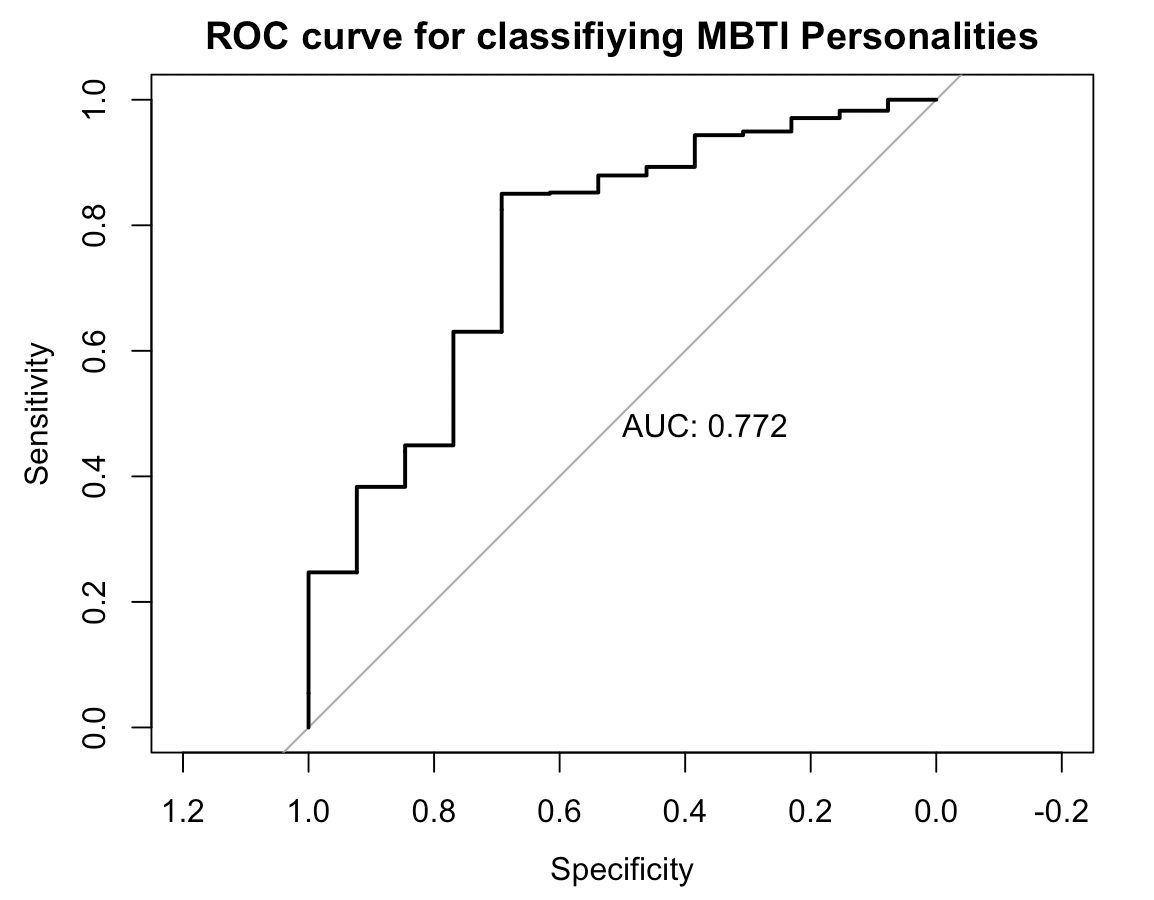
\includegraphics[scale=0.4]{ROC.png}
\caption{Aggregated ROC curve for the multi-class SVM.} %explain multi-class
\label{fig:ROC}
\end{figure}

All SVMs yielded considerably higher results than the baseline. The \textit{text + features} model was able to classify 62\% of people's personality types in the test set correctly, the robust and unbiased model 54\%, see figure \ref{fig:Pred}. This result including a well-shaped ROC curve, figure \ref{fig:ROC}, answers that at least for this dataset the MBTI can be predicted (1). The confusion matrix shows how the prior distribution of personality types influenced the result: most classification errors happened in the more frequent categories among the over-represented introverts. Interestingly, especially the personality types that differ only in one dimension are more often missclassified. This could imply a general validity of the MBTI (2): types that don't have much resemblance in theory are usually not confused here either.
\begin{figure}[b]
\centering
    \begin{subfigure}[b]{.6\textwidth}
      %\centering
      \raggedright
      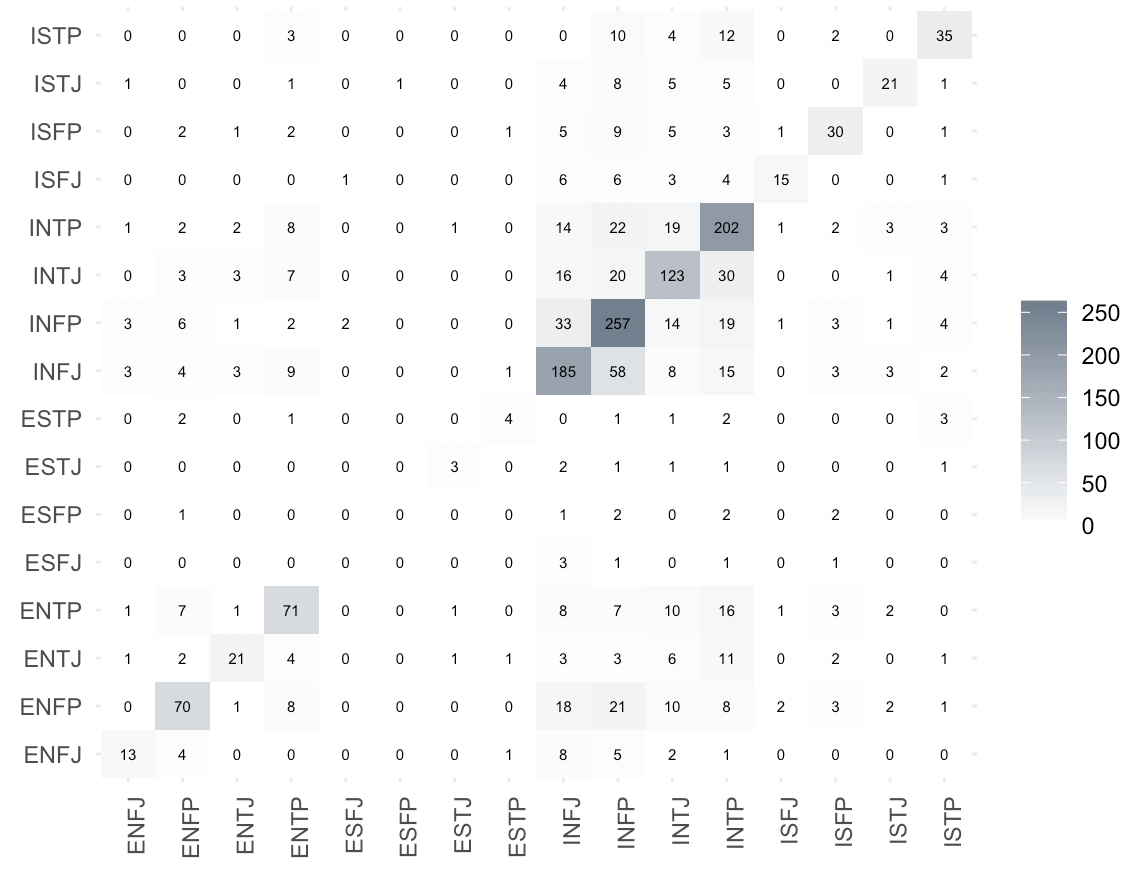
\includegraphics[width=\textwidth]{confusionmatrixlabels.png}
        \caption{Confusion Matrix} %explain more
        \label{fig:Conf}
    \end{subfigure}%
    \quad %spacing between figures
    \begin{subfigure}[b]{.35\textwidth}
        %\begin{table}
        \raggedleft
        \label{tab:Pred}
        \begin{tabular}{ll}
            \hline\noalign{\smallskip}
            \textbf{Model} & \\
            \noalign{\smallskip}\hline\noalign{\smallskip}
            plain features & 0.21 \\
            plain text & 0.56 \\
            text + features & 0.62 \\
            \noalign{\smallskip}\hline\noalign{\smallskip}
            \textit{text + features +} & \\
            unbiased w/o type & 0.46 \\
            robust 7 classes & 0.54 \\
            robust + unbiased & 0.54 \\
            %\noalign{\smallskip}\hline\noalign{\smallskip}
            \noalign{\smallskip}\hline
            \\ \\
        \end{tabular}
        \caption{Prediction accuracy}
        %\end{table}
    \end{subfigure}
    \caption{Prediction results}
    \label{fig:Pred}
\end{figure}
The \textit{plain features} model comes to 21\%. If only the features were used for prediction, they would have to be improved to perform well. As however the personality types are predicted from text, the features may still add some points in accuracy to the model: The text by itself comes to 56\%, with features it is 62\% accurate.\\
This result is unfortunately biased. As predicted, mentioning one's own personality even without referring to oneself has a big impact on the model's performance: if one's own personality type is removed from text, it results in a dropped accuracy of 46\%. If however it is altered to a more robust model with the stable classes, it comes to a promising 54\%. Overall, this supports the notion of the MBTI being predictable here and indicates proof for research question (1).